\documentclass[12pt]{article}
 
\usepackage[table]{xcolor}
\usepackage[margin=1in]{geometry} 
\usepackage{amsmath,amsthm,amssymb,wasysym}
\usepackage{pgf,tikz,pgfplots}
\usepackage{mathrsfs}
\usepackage{mathtools}
\usepackage{listings}
\usepackage{colortbl}
\usepackage{verbatim}
\usetikzlibrary{arrows, angles, quotes, decorations.pathreplacing, math, patterns}
\usepackage{framed}

\lstset{basicstyle=\footnotesize}
\usetikzlibrary{calc}

\newcommand{\N}{\mathbb{N}}
\newcommand{\Z}{\mathbb{Z}}
\newcommand{\I}{\mathbb{I}}
\newcommand{\R}{\mathbb{R}}
\newcommand{\Q}{\mathbb{Q}}
\DeclarePairedDelimiter{\ceil}{\lceil}{\rceil}
 
\begin{document}
 
\title{Coloring\\
    \large CS101A Problem Solving I}
\author{Harry Coleman}
\date{November 5, 2019}

\maketitle

\section*{Problem 2}
\fbox{
    \parbox{\textwidth} {
        Show that $n$ points $(n \geq 5)$ of the plane can be colored by two colors so that no line can separate the points of one color from those of the other color.
    }
}
\\

To show that it is always possible to color $n \geq 5$ points such that no line can separate the points of one color from those of the other color, we're going to look at three cases. Given any set of $n \geq 5$ points on a plane, we know there must be at least four points. If any three of these points are collinear, we can color them in the following way.

\begin{center}
    
\begin{tikzpicture}
        \coordinate (A) at (0,0);
        \coordinate (B) at (1,0);
        \coordinate (C) at (2,0);
        
        \draw[black] (A) circle (5pt);
        \filldraw[black] (B) circle (5pt);
        \draw[black] (C) circle (5pt);
    \end{tikzpicture}
\end{center}

Clearly, no line could be drawn to separate the black point from the black point. If there are no three collinear points, then three points must form a triangle.

\begin{center}
    \begin{tikzpicture}
        \coordinate (A) at (0,0);
        \coordinate (B) at (2,0);
        \coordinate (C) at (1,1.5);
        
        \draw[black] (A) circle (5pt);
        \draw[black] (B) circle (5pt);
        \draw[black] (C) circle (5pt);
    \end{tikzpicture}
\end{center}

Our fourth point must lie in the interior or exterior of this triangle. Either of these cases can be colored such that no line can be draw to separate black and white points.
\begin{center}
    \begin{tikzpicture}
        \coordinate (A) at (0,0);
        \coordinate (B) at (2,0);
        \coordinate (C) at (1,1.5);
        \coordinate (D) at (-.5,1.5);
        
        \draw[black] (A) circle (5pt);
        \filldraw[black] (B) circle (5pt);
        \draw[black] (C) circle (5pt);
        \filldraw[black] (D) circle (5pt);
        
        \draw[dashed] (3,-0.5) -- (3,2.5);
        
        \coordinate (E) at (4,0);
        \coordinate (F) at (6,0);
        \coordinate (G) at (5,1.5);
        \coordinate (H) at (5,.5);
        
        \draw[black] (E) circle (5pt);
        \draw[black] (F) circle (5pt);
        \draw[black] (G) circle (5pt);
        \filldraw[black] (H) circle (5pt);
    \end{tikzpicture}
\end{center}

This means that any collection of $n\geq5$ points can be colored such that no line can be drawn which separates black and white points.




\newpage
\section*{Problem 3}
\fbox{
    \parbox{\textwidth} {
         Is there a way to pack 250 $1 \times 1 \times 4$ bricks into a $10 \times 10 \times 10$ box?
    }
}
\\

We'll color $10 \times 10 \times 10$ box by alternating black and white $2 \times 2 \times 2$ boxes. A 2-dimensional cross-section would look like a checkerboard.
\begin{center}
    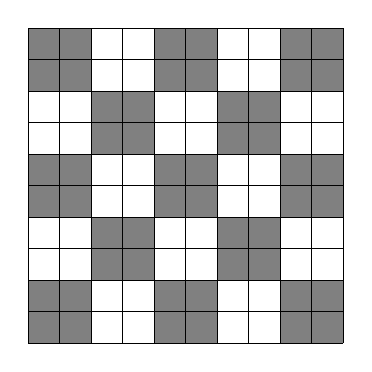
\begin{tikzpicture}
        \fill[gray] (0,0) rectangle (.8,.8);
        \fill[gray] (1.6,0) rectangle (2.4,.8);
        \fill[gray] (3.2,0) rectangle (4,.8);
        \fill[gray] (0,1.6) rectangle (.8,2.4);
        \fill[gray] (1.6,1.6) rectangle (2.4,2.4);
        \fill[gray] (3.2,1.6) rectangle (4,2.4);
        \fill[gray] (0,3.2) rectangle (.8,4);
        \fill[gray] (1.6,3.2) rectangle (2.4,4);
        \fill[gray] (3.2,3.2) rectangle (4,4);
        \fill[gray] (.8,.8) rectangle (1.6,1.6);
        \fill[gray] (2.4,.8) rectangle (3.2,1.6);
        \fill[gray] (.8,2.4) rectangle (1.6,3.2);
        \fill[gray] (2.4,2.4) rectangle (3.2,3.2);
        
       
        \draw[step=.4cm,thin] (0,0) grid (4,4);
    \end{tikzpicture}
\end{center}

If we place a $1 \times 1 \times 4$ brick inside this colored box, it will always take up equal black to white volume.

\begin{center}
    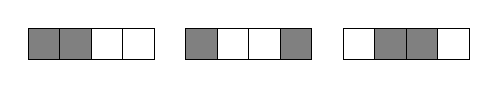
\begin{tikzpicture}
        \fill[gray] (0,0) rectangle (.8,.4);
        
        \fill[gray] (2,0) rectangle (2.4,.4);
        \fill[gray] (3.2,0) rectangle (3.6,.4);
        
        \fill[gray] (4.4,0) rectangle (5.2,.4);
        
        \draw[step=.4cm,thin] (0,0) grid (1.6,.4);
        \draw[step=.4cm,thin] (1.999,0) grid (3.6,.4);
        \draw[step=.4cm,thin] (3.999,0) grid (5.6,.4);
    \end{tikzpicture}
\end{center}

However, the $10\times10\times10$ box, colored in this way, has 8 more black volume units than white volume units. Therefore, we cannot pack the bricks into the box.


\section*{Problem 4}
\fbox{
    \parbox{\textwidth} {
         A beetle sits on each square of a $9\times9$ chessboard. At a signal each beetle crawls diagonally onto a neighboring square. Then it may happen that several beetles will sit on some squares and none on others. Find the minimal possible number of free squares
    }
}
\\

Each beetle can only move to an adjacent diagonal square. In the following diagram, each beetle starting on a light gray square can only move to a dark gray square, and vice versa. 

\begin{center}
    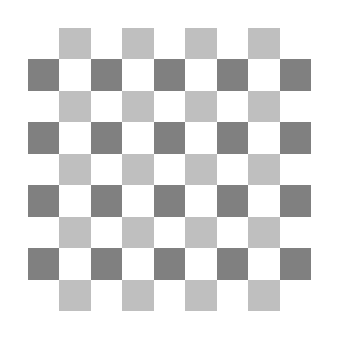
\begin{tikzpicture}
        \foreach \x in {.4,1.2,2,2.8} {
            \foreach \y in {0,.8,1.6,2.4,3.2} {
                \fill[gray!50] (\x,\y) rectangle (\x+.4,\y+.4);
            }
        }
        \foreach \x in {0,.8,1.6,2.4,3.2} {
            \foreach \y in {.4,1.2,2,2.8} {
                \fill[gray] (\x,\y) rectangle (\x+.4,\y+.4);
            }
        }
    \end{tikzpicture}
\end{center}

We'll show one possible combination of movements. A line between two squares represents the beetles from each square swapping positions.

\begin{center}
    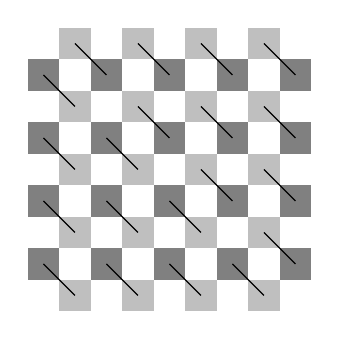
\begin{tikzpicture}
        \foreach \x in {.4,1.2,2,2.8} {
            \foreach \y in {0,.8,1.6,2.4,3.2} {
                \fill[gray!50] (\x,\y) rectangle (\x+.4,\y+.4);
            }
        }
        \foreach \x in {0,.8,1.6,2.4,3.2} {
            \foreach \y in {.4,1.2,2,2.8} {
                \fill[gray] (\x,\y) rectangle (\x+.4,\y+.4);
            }
        }
        \draw (.2,.6) -- (.6,.2);
        \draw (.2,1.4) -- (.6,1);
        \draw (.2,2.2) -- (.6,1.8);
        \draw (.2,3) -- (.6,2.6);
        
        \draw (1,.6) -- (1.4,.2);
        \draw (1,1.4) -- (1.4,1);
        \draw (1,2.2) -- (1.4,1.8);
        
        \draw (1.8,.6) -- (2.2,.2);
        \draw (1.8,1.4) -- (2.2,1);
        
        \draw (2.6,.6) -- (3,.2);
        
        \draw (.6,3.4) -- (1,3);
        
        \draw (1.4,3.4) -- (1.8,3);
        \draw (1.4,2.6) -- (1.8,2.2);
        
        \draw (2.2,3.4) -- (2.6,3);
        \draw (2.2,2.6) -- (2.6,2.2);
        \draw (2.2,1.8) -- (2.6,1.4);
        
        \draw (3,3.4) -- (3.4,3);
        \draw (3,2.6) -- (3.4,2.2);
        \draw (3,1.8) -- (3.4,1.4);
        \draw (3,1) -- (3.4,.6);
    \end{tikzpicture}
\end{center}

So for those squares, we can have zero free squares after movement. The other set of squares on the board have the same property that every beetle on a light gray square moves to a dark gray square, and vice versa.

\begin{center}
    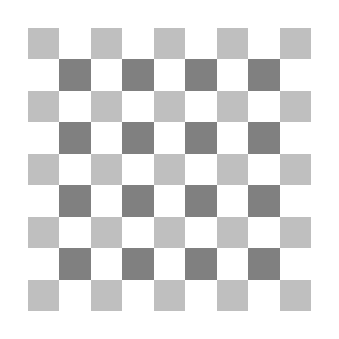
\begin{tikzpicture}
        \foreach \x in {0,.8,1.6,2.4,3.2} {
            \foreach \y in {0,.8,1.6,2.4,3.2} {
                \fill[gray!50] (\x,\y) rectangle (\x+.4,\y+.4);
            }
        }
        \foreach \x in {.4,1.2,2,2.8} {
            \foreach \y in {.4,1.2,2,2.8} {
                \fill[gray] (\x,\y) rectangle (\x+.4,\y+.4);
            }
        }
    \end{tikzpicture}
\end{center}

For these squares, we can have the beetles perform a similar pattern of movement.

\begin{center}
    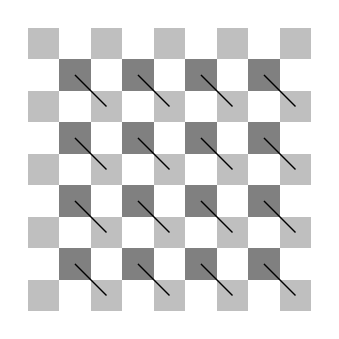
\begin{tikzpicture}
        \foreach \x in {0,.8,1.6,2.4,3.2} {
            \foreach \y in {0,.8,1.6,2.4,3.2} {
                \fill[gray!50] (\x,\y) rectangle (\x+.4,\y+.4);
            }
        }
        \foreach \x in {.4,1.2,2,2.8} {
            \foreach \y in {.4,1.2,2,2.8} {
                \fill[gray] (\x,\y) rectangle (\x+.4,\y+.4);
            }
        }
        \draw (.6,.6) -- (1,.2);
        \draw (.6,1.4) -- (1,1);
        \draw (.6,2.2) -- (1,1.8);
        \draw (.6,3) -- (1,2.6);
        
        \draw (1.4,.6) -- (1.8,.2);
        \draw (1.4,1.4) -- (1.8,1);
        \draw (1.4,2.2) -- (1.8,1.8);
        
        \draw (2.2,.6) -- (2.6,.2);
        \draw (2.2,1.4) -- (2.6,1);
        
        \draw (3,.6) -- (3.4,.2);
        
        \draw (1.4,3) -- (1.8,2.6);
        
        \draw (2.2,3) -- (2.6,2.6);
        \draw (2.2,2.2) -- (2.6,1.8);
        
        \draw (3,3) -- (3.4,2.6);
        \draw (3,2.2) -- (3.4,1.8);
        \draw (3,1.4) -- (3.4,1);
    \end{tikzpicture}
\end{center}

However, we find that since there are more light gray squares than dark gray squares, we can have all of the dark gray end up covered, but we can only end up with a number of light gray squares covered equal to the number of dark gray squares. Since there are nine more light gray squares than dark gray squares, we must have at least nine light gray squares free after movement. Meaning that the minimal number of free squares is 9.

\newpage
\section*{Problem 5}
\fbox{
    \parbox{\textwidth} {
        An art gallery has the shape of a simple n-gon. Find the minimum number of watchmen needed to survey the building, no matter how complicated its shape.
    }
}
\\

Any triangle can be surveyed by one watchman at any point in or on the triangle. We'll assume that a watchman,$\CIRCLE$, can be placed directly at a corner.
\begin{center}
    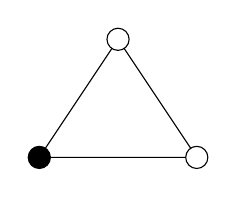
\begin{tikzpicture}
        \draw[] (0,0)--(2,0)--(1,1.5)--(0,0);
        
        \draw[fill=black] (0,0) circle (4pt);
        \draw[fill=white] (2,0) circle (4pt);
        \draw[fill=white] (1,1.5) circle (4pt);
    \end{tikzpicture}
\end{center}

We can divide any simple $n$-gon into a collection of $(n-2)$ triangles.
\begin{center}
    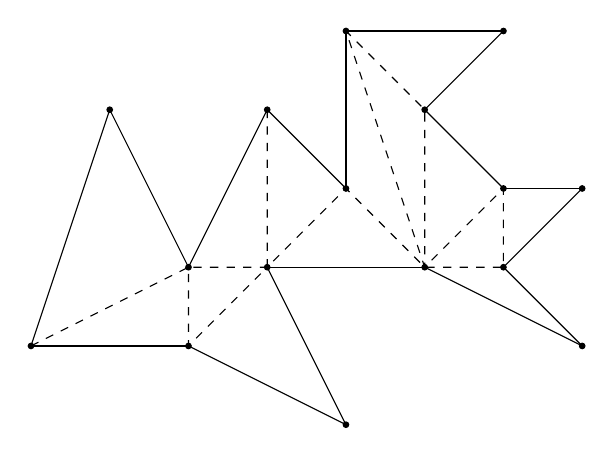
\begin{tikzpicture}
        \draw[] (0,1)-- (1,4);
        \draw[] (1,4)-- (2,2);
        \draw[] (2,2)-- (3,4);
        \draw[] (3,4)-- (4,3);
        \draw[] (4,3)-- (4,5);
        \draw[] (4,5)-- (6,5);
        \draw[] (6,5)-- (5,4);
        \draw[] (5,4)-- (6,3);
        \draw[] (6,3)-- (7,3);
        \draw[] (7,3)-- (6,2);
        \draw[] (6,2)-- (7,1);
        \draw[] (7,1)-- (5,2);
        \draw[] (5,2)-- (3,2);
        \draw[] (3,2)-- (4,0);
        \draw[] (4,0)-- (2,1);
        \draw[] (2,1)-- (0,1);
        \draw[fill=black] (0,1) circle (1pt);
        \draw[fill=black] (1,4) circle (1pt);
        \draw[fill=black] (3,4) circle (1pt);
        \draw[fill=black] (4,3) circle (1pt);
        \draw[fill=black] (4,5) circle (1pt);
        \draw[fill=black] (6,5) circle (1pt);
        \draw[fill=black] (5,4) circle (1pt);
        \draw[fill=black] (6,3) circle (1pt);
        \draw[fill=black] (7,3) circle (1pt);
        \draw[fill=black] (6,2) circle (1pt);
        \draw[fill=black] (7,1) circle (1pt);
        \draw[fill=black] (5,2) circle (1pt);
        \draw[fill=black] (4,0) circle (1pt);
        \draw[fill=black] (2,1) circle (1pt);
        \draw[fill=black] (3,2) circle (1pt);
        \draw[fill=black] (2,2) circle (1pt);
        
        \draw[dashed] (0,1)--(2,2)--(2,1)--(3,2)--(2,2);
        \draw[dashed] (3,4)--(3,2)--(4,3)--(5,2)--(6,2)--(6,3)--(5,2)--(4,5)--(5,4)--(5,2);
    \end{tikzpicture}
\end{center}

Any three adjacent triangles share exactly one vertex. A watchman placed at this shared vertex could see all three triangles, no matter their shape.
\begin{center}
    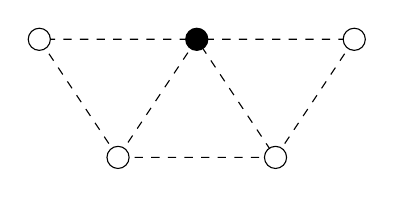
\begin{tikzpicture}
        \draw[dashed] (0,0)--(2,0)--(1,1.5)--(0,0);
        \draw[dashed] (0,0)--(-1,1.5)--(1,1.5);
        \draw[dashed] (2,0)--(3,1.5)--(1,1.5);
        
        \draw[fill=white] (0,0) circle (4pt);
        \draw[fill=white] (2,0) circle (4pt);
        \draw[fill=black] (1,1.5) circle (4pt);
        \draw[fill=white] (-1,1.5) circle (4pt);
        \draw[fill=white] (3,1.5) circle (4pt);
    \end{tikzpicture}
\end{center}

Since we have $n-2$ triangles, we can form $\ceil[\big]{\frac{n-2}{3}}$ groups of three triangles. (If $n-2$ is not a multiple of 3, then one of the groups will have one or two triangles.) So $\ceil[\big]{\frac{n-2}{3}}$ watchmen is always sufficient to survey the building. To show that for all $n$, $\ceil[\big]{\frac{n-2}{3}}$ watchmen is sometimes necessary, we'll provide a General form for constructing a building of greatest survey complexity.

\definecolor{wrwrwr}{rgb}{0.3803921568627451,0.3803921568627451,0.3803921568627451}
\begin{center}
    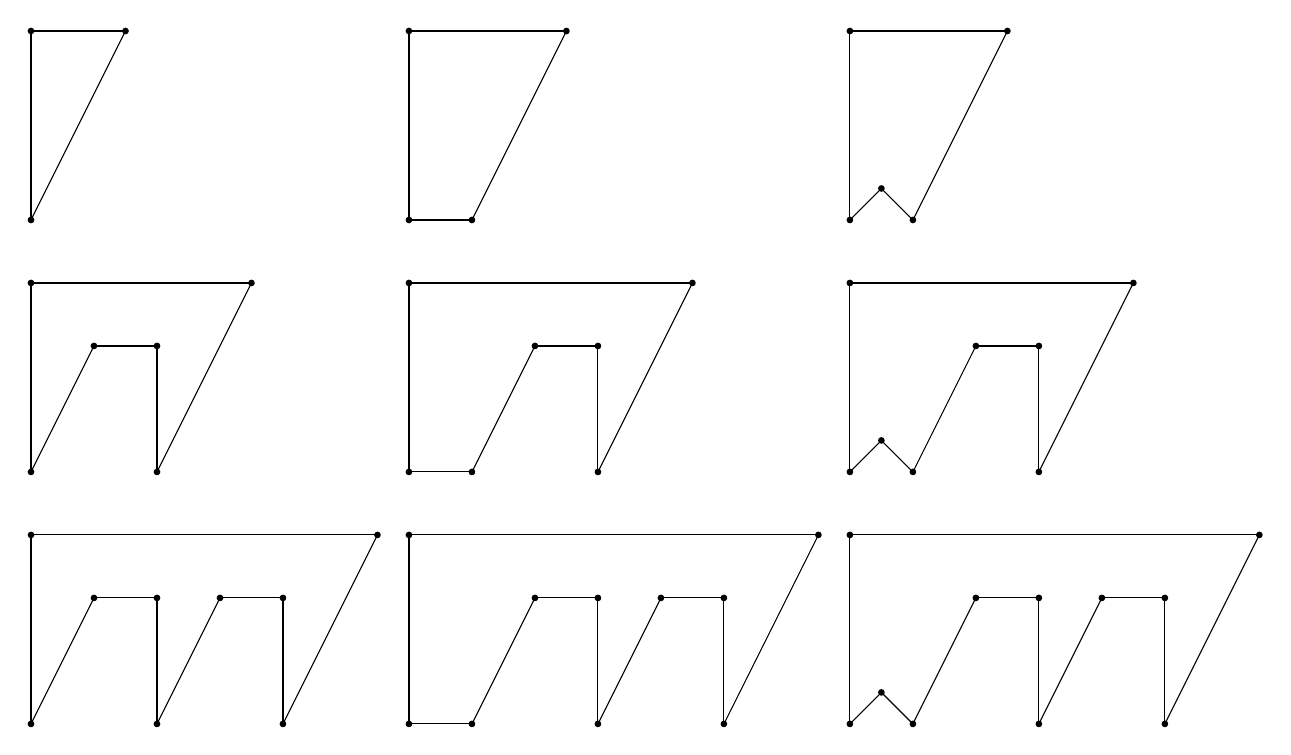
\begin{tikzpicture}[line cap=round,line join=round,>=triangle 45,x=.8cm,y=.8cm]
        \draw [] (0,0)-- (0,3);
        \draw [] (0,3)-- (1.5,3);
        \draw [] (1.5,3)-- (0,0);
        \draw [] (0,-1)-- (0,-4);
        \draw [] (0,-4)-- (1,-2);
        \draw [] (1,-2)-- (2,-2);
        \draw [] (2,-2)-- (2,-4);
        \draw [] (2,-4)-- (3.5,-1);
        \draw [] (3.5,-1)-- (0,-1);
        \draw [] (0,-5)-- (0,-8);
        \draw [] (0,-8)-- (1,-6);
        \draw [] (1,-6)-- (2,-6);
        \draw [] (2,-6)-- (2,-8);
        \draw [] (2,-8)-- (3,-6);
        \draw [] (3,-6)-- (4,-6);
        \draw [] (4,-6)-- (4,-8);
        \draw [] (4,-8)-- (5.5,-5);
        \draw [] (5.5,-5)-- (0,-5);
        \draw [] (6,3)-- (6,0);
        \draw [] (6,0)-- (7,0);
        \draw [] (7,0)-- (8.5,3);
        \draw [] (8.5,3)-- (6,3);
        \draw [] (6,-1)-- (6,-4);
        \draw [] (6,-4)-- (7,-4);
        \draw [] (7,-4)-- (8,-2);
        \draw [] (8,-2)-- (9,-2);
        \draw [] (9,-2)-- (9,-4);
        \draw [] (9,-4)-- (10.5,-1);
        \draw [] (10.5,-1)-- (6,-1);
        \draw [] (6,-5)-- (6,-8);
        \draw [] (6,-8)-- (7,-8);
        \draw [] (7,-8)-- (8,-6);
        \draw [] (8,-6)-- (9,-6);
        \draw [] (9,-6)-- (9,-8);
        \draw [] (9,-8)-- (10,-6);
        \draw [] (10,-6)-- (11,-6);
        \draw [] (11,-6)-- (11,-8);
        \draw [] (11,-8)-- (12.5,-5);
        \draw [] (12.5,-5)-- (6,-5);
        \draw [] (13,3)-- (13,0);
        \draw [] (13,0)-- (13.5,0.5);
        \draw [] (13.5,0.5)-- (14,0);
        \draw [] (14,0)-- (15.5,3);
        \draw [] (15.5,3)-- (13,3);
        \draw [] (13,-1)-- (13,-4);
        \draw [] (13,-4)-- (13.5,-3.5);
        \draw [] (13.5,-3.5)-- (14,-4);
        \draw [] (14,-4)-- (15,-2);
        \draw [] (15,-2)-- (16,-2);
        \draw [] (16,-2)-- (16,-4);
        \draw [] (16,-4)-- (17.5,-1);
        \draw [] (17.5,-1)-- (13,-1);
        \draw [] (13,-5)-- (13,-8);
        \draw [] (13,-8)-- (13.5,-7.5);
        \draw [] (13.5,-7.5)-- (14,-8);
        \draw [] (14,-8)-- (15,-6);
        \draw [] (15,-6)-- (16,-6);
        \draw [] (16,-6)-- (16,-8);
        \draw [] (16,-8)-- (17,-6);
        \draw [] (17,-6)-- (18,-6);
        \draw [] (18,-6)-- (18,-8);
        \draw [] (18,-8)-- (19.5,-5);
        \draw [] (19.5,-5)-- (13,-5);
        \draw [fill=black] (0,0) circle (1pt);
        \draw [fill=black] (0,3) circle (1pt);
        \draw [fill=black] (1.5,3) circle (1pt);
        \draw [fill=black] (0,-1) circle (1pt);
        \draw [fill=black] (0,-4) circle (1pt);
        \draw [fill=black] (1,-2) circle (1pt);
        \draw [fill=black] (2,-2) circle (1pt);
        \draw [fill=black] (2,-4) circle (1pt);
        \draw [fill=black] (3.5,-1) circle (1pt);
        \draw [fill=black] (0,-5) circle (1pt);
        \draw [fill=black] (0,-8) circle (1pt);
        \draw [fill=black] (1,-6) circle (1pt);
        \draw [fill=black] (2,-6) circle (1pt);
        \draw [fill=black] (2,-8) circle (1pt);
        \draw [fill=black] (3,-6) circle (1pt);
        \draw [fill=black] (4,-6) circle (1pt);
        \draw [fill=black] (4,-8) circle (1pt);
        \draw [fill=black] (5.5,-5) circle (1pt);
        \draw [fill=black] (6,3) circle (1pt);
        \draw [fill=black] (6,0) circle (1pt);
        \draw [fill=black] (7,0) circle (1pt);
        \draw [fill=black] (8.5,3) circle (1pt);
        \draw [fill=black] (6,-1) circle (1pt);
        \draw [fill=black] (6,-4) circle (1pt);
        \draw [fill=black] (7,-4) circle (1pt);
        \draw [fill=black] (8,-2) circle (1pt);
        \draw [fill=black] (9,-2) circle (1pt);
        \draw [fill=black] (9,-4) circle (1pt);
        \draw [fill=black] (10.5,-1) circle (1pt);
        \draw [fill=black] (6,-5) circle (1pt);
        \draw [fill=black] (6,-8) circle (1pt);
        \draw [fill=black] (7,-8) circle (1pt);
        \draw [fill=black] (8,-6) circle (1pt);
        \draw [fill=black] (9,-6) circle (1pt);
        \draw [fill=black] (9,-8) circle (1pt);
        \draw [fill=black] (10,-6) circle (1pt);
        \draw [fill=black] (11,-6) circle (1pt);
        \draw [fill=black] (11,-8) circle (1pt);
        \draw [fill=black] (12.5,-5) circle (1pt);
        \draw [fill=black] (13,3) circle (1pt);
        \draw [fill=black] (13,0) circle (1pt);
        \draw [fill=black] (13.5,0.5) circle (1pt);
        \draw [fill=black] (14,0) circle (1pt);
        \draw [fill=black] (15.5,3) circle (1pt);
        \draw [fill=black] (13,-1) circle (1pt);
        \draw [fill=black] (13,-4) circle (1pt);
        \draw [fill=black] (13.5,-3.5) circle (1pt);
        \draw [fill=black] (14,-4) circle (1pt);
        \draw [fill=black] (15,-2) circle (1pt);
        \draw [fill=black] (16,-2) circle (1pt);
        \draw [fill=black] (16,-4) circle (1pt);
        \draw [fill=black] (17.5,-1) circle (1pt);
        \draw [fill=black] (13,-5) circle (1pt);
        \draw [fill=black] (13,-8) circle (1pt);
        \draw [fill=black] (13.5,-7.5) circle (1pt);
        \draw [fill=black] (14,-8) circle (1pt);
        \draw [fill=black] (15,-6) circle (1pt);
        \draw [fill=black] (16,-6) circle (1pt);
        \draw [fill=black] (16,-8) circle (1pt);
        \draw [fill=black] (17,-6) circle (1pt);
        \draw [fill=black] (18,-6) circle (1pt);
        \draw [fill=black] (18,-8) circle (1pt);
        \draw [fill=black] (19.5,-5) circle (1pt);
    \end{tikzpicture}
\end{center}

We could continue each row arbitrarily to find an $n-gon$ which requires $\ceil[\big]{\frac{n-2}{3}}$ watchmen. So for any $n$-gon, $\ceil[\big]{\frac{n-2}{3}}$ is a sufficient and sometimes necessary number of watchmen.

\newpage
\section*{Problem 6}
\fbox{
    \parbox{\textwidth} {
        Every (3D) space point is colored either red or blue. Show that among the squares with side 1 in this space there is at least one with three red vertices or at least one with four blue vertices.
    }
}
\\

To show that there must be at least one unit square with red vertices or at least one unit square with four blue vertices, we'll assume that it is possible to color the 3D space in such a way that neither of these two types of squares exist.

This means that the only squares that can exist are the following.
\begin{align*}
    \text{Red} &= \CIRCLE \\
    \text{Blue} &= \Circle\\
\end{align*}
\begin{center}
    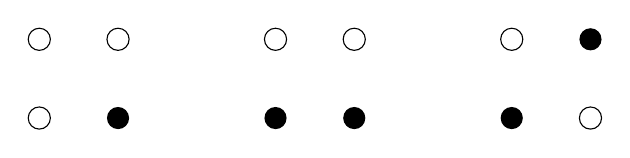
\begin{tikzpicture}
        \draw[black] (0,0) circle (4pt);
        \fill[black] (1,0) circle (4pt);
        \draw[black] (0,1) circle (4pt);
        \draw[black] (1,1) circle (4pt);
        
        \fill[black] (3,0) circle (4pt);
        \fill[black] (4,0) circle (4pt);
        \draw[black] (3,1) circle (4pt);
        \draw[black] (4,1) circle (4pt);
        
        \fill[black] (6,0) circle (4pt);
        \draw[black] (7,0) circle (4pt);
        \draw[black] (6,1) circle (4pt);
        \fill[black] (7,1) circle (4pt);
    \end{tikzpicture}
\end{center}

If the whole space were colored blue, then of course there would be a unit square with four blue vertices, so there must exist at least one red point.
\begin{center}
    
\begin{tikzpicture}
        \fill[black] (0,0) circle (4pt);
    \end{tikzpicture}
\end{center}

Around this red point, we consider a sphere of radius 1 unit. If the sphere were entirely blue, it would be trivial to find a unit square on the surface of the sphere with four blue vertices. So there must be at least one red point on the sphere. This means there is two red points that are 1 unit apart.
\begin{center}
    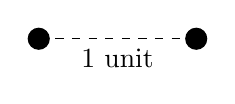
\begin{tikzpicture}
        \fill[black] (0,0) circle (4pt);
        \fill[black] (2,0) circle (4pt);
        
        \draw[dashed] (0,0) -- (2,0) node[midway, anchor=north] {1 unit};
    \end{tikzpicture}
\end{center}

We now consider 4 more points which, together with the two red points, form an equilateral triangular prism where all edges are 1 unit.
\begin{center}
    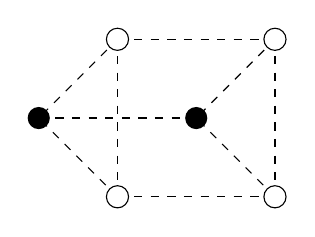
\begin{tikzpicture}
        \coordinate (A) at (0,0);
        \coordinate (B) at (2,0);
        \coordinate (C) at (1,1);
        \coordinate (D) at (1,-1);
        \coordinate (E) at (3,1);
        \coordinate (F) at (3,-1);
        
        \draw[dashed] (A) -- (B);
        \draw[dashed] (C) -- (D);
        \draw[dashed] (E) -- (F);
        \draw[dashed] (C) -- (E);
        \draw[dashed] (D) -- (F);
        
        \draw[dashed] (D) -- (A) -- (C);
        \draw[dashed] (F) -- (B) -- (E);
        
        \fill[black] (A) circle (4pt);
        \fill[black] (B) circle (4pt);
        \draw[fill=white] (C) circle (4pt);
        \draw[fill=white] (D) circle (4pt);
        \draw[fill=white] (E) circle (4pt);
        \draw[fill=white] (F) circle (4pt);
    \end{tikzpicture}
\end{center}

Currently, we see a unit square with four blue vertices, since this is not allowed, we must color one of these red.
\begin{center}
    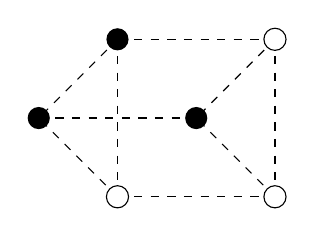
\begin{tikzpicture}
        \coordinate (A) at (0,0);
        \coordinate (B) at (2,0);
        \coordinate (C) at (1,1);
        \coordinate (D) at (1,-1);
        \coordinate (E) at (3,1);
        \coordinate (F) at (3,-1);
        
        \draw[dashed] (A) -- (B);
        \draw[dashed] (C) -- (D);
        \draw[dashed] (E) -- (F);
        \draw[dashed] (C) -- (E);
        \draw[dashed] (D) -- (F);
        
        \draw[dashed] (D) -- (A) -- (C);
        \draw[dashed] (F) -- (B) -- (E);
        
        \fill[black] (A) circle (4pt);
        \fill[black] (B) circle (4pt);
        \fill[black] (C) circle (4pt);
        \draw[fill=white] (D) circle (4pt);
        \draw[fill=white] (E) circle (4pt);
        \draw[fill=white] (F) circle (4pt);
    \end{tikzpicture}
\end{center}

This, however, produces a unit square with three red vertices. Either of these situations contradict our initial assumption. Therefore, in a red and blue colored 3D point space, we must have at least one unit square with four blue vertices or at least one unit square with three red vertices.

\newpage
\section*{Problem 7}
\fbox{
    \parbox{\textwidth} {
        All vertices of a convex pentagon are lattice points (have integral coordinates), and its sides have integral length. Show that its perimeter is even.
    }
}
\\

We will color all the lattice points in our plane. Each point, $(x,y)$, will be colored
\begin{center}
    black if $x+y$ is even
    
    white if $x+y$ is odd
\end{center}
so the plane is a sort of checkerboard.
\begin{center}
    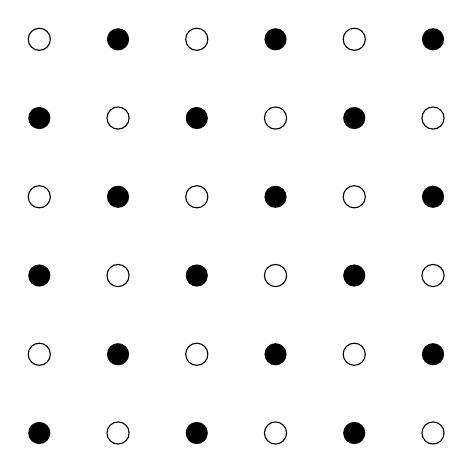
\begin{tikzpicture}
        \foreach \x in {1,3,5} {
            \foreach \y in {0,2,4} {
                \draw[black] (\x,\y) circle (4pt);
                \draw[black] (\y,\x) circle (4pt);
            }
        }
        \foreach \x in {0,2,4} {
            \foreach \y in {0,2,4} {
                \fill[black] (\x,\y) circle (4pt);
                \fill[black] (\x+1,\y+1) circle (4pt);
            }
        }
    \end{tikzpicture}
\end{center}

Since each vertex of our pentagon is a lattice point, we'll consider each side to be the hypotenuse of a right triangle. For any two vertices, $A$ and $B$, of the pentagon, there is a horizontal displacement, $\Delta x$, a vertical displacement, $\Delta y$, and a side length, $d$, all of which are integral.
\begin{center}
    \begin{tikzpicture}
        \coordinate (A) at (0,0);
        \coordinate (B) at (4,3);
        \coordinate (C) at (4,0);
        
        \draw (A) node[anchor=east]{$A$}; 
        \draw (B) node[anchor=west]{$B$}; 
        
        \draw[black] (A) -- (B) node[midway, anchor=south east] {$d$};
        \draw[dashed] (A) -- (C) node[midway, anchor=north] {$\Delta x$};
        \draw[dashed] (B) -- (C) node[midway, anchor=west] {$\Delta y$};
        
        \draw[black] (3.7,0)--(3.7,.3)--(4,.3);
    \end{tikzpicture}
\end{center}

Applying this to our coloring, we know that the coloring of any two points $A$ and $B$ is the same if and only if $\Delta x$ and $\Delta y$ have the same parity.

Since $A$ and $B$ are lattice points, and $d$ is an integer, we can use the properties of Pythagorean triples of $(\Delta x, \Delta y, d)$. So $(\Delta x)^2 + (\Delta y)^2 = d^2$. This means that $d$ is even if and only if $\Delta x$ and $\Delta y$ have the same parity.
\begin{center}
    \rowcolors{1}{gray!10}{white}
    \begin{tabular}{cc|c}
        \multicolumn{2}{c}{Parity} & \multicolumn{1}{c}{Coloring} \\
        $\Delta x$ $\Delta y$ & $d$ & $A$  $B$\\
        \hline
        same & even & same \\
        opposite & odd & opposite \\
    \end{tabular}
\end{center}

So the coloring of $A$ and $B$ is the same if and only if $d$ is even. Consider now, an arbitrary pentagon $ABCDE$. If we list the vertex colors starting and ending at $A$, we get a sequence of black and white points. For example, we might have the sequence
\begin{center}
    \begin{tabular}{cccccc}
        $A$ & $B$ & $C$ & $D$ & $E$ & $A$ \\
        \hline
        $\CIRCLE$ & $\Circle$ & $\Circle$ & $\CIRCLE$ & $\Circle$ & $\CIRCLE$
    \end{tabular}
\end{center}

Since the sequence must begin and end on black, every pair $\CIRCLE \Circle$ must eventually be followed by the pair $\Circle \CIRCLE$. (Starting on white, we would reverse the two pairs.) Because of this symmetry, we will always have an even number of pairs with opposite color.

This means we must have an even number of odd side lengths, giving us an even perimeter. In fact, this means any polygon with lattice point vertices must have an even perimeter, not just convex pentagons.


\section*{Problem 8}
\fbox{
    \parbox{\textwidth} {
         Consider three vertices $A = (0, 0)$, $B = (0, 1)$, $C = (1, 0)$ in a plane lattice. Can you reach the fourth vertex $D = (1, 1)$ of the square by reflections at $A$, $B$, $C$ or at points previously reflected?
    }
}
\\

The only operation we can perform is a point reflection. This means that if we are given two points $(x, y), (a, b)$, we can obtain the reflection of $(x,y)$ at $(a,b)$ by
\begin{align*}
    x^\prime &= x+2(a-x) \\
    y^\prime &=  y+2(b-y)
\end{align*}
and our new point is $(x^\prime, y^\prime)$. If $(x,y)$ and $(a,b)$ are lattice points, $(x^\prime, y^\prime)$ is also a lattice points. Since we are starting with $A, B, C$ that are lattice points, all new points obtained by reflection will also be lattice points.

We can see from the above equations, that we are  adding a multiple of 2 to each $x$ and $y$, this means that the parity of $x$ and $y$ do not change when reflected across a lattice point. Looking at our given points, we have
\begin{alignat*}{3}
    A &= (0,0) &&= \text{(even, even)} \\
    B &= (0,1) &&= \text{(even, odd)} \\
    C &= (1,0) &&= \text{(odd, even)} 
\end{alignat*}

This means that every point that can be obtained by reflection will have one of the three above parities. However, since
\[D = (1,1) = \text{(odd, odd)}\]
D cannot be one of the points obtainable by reflection.


 
\end{document}